\chapter{Design and Implementation}
\label{Implementation}

This chapter describes the Design process and the details of the realised implementation of a Docker based application developed for managing ROS2 Nodes in a local Network over a web interface. Figure \ref*{fig:Background:LifecycleManagement} provides an overview of the Structure of the developed Application. The Application is supposed to have control over all the compatible ROS2 Applications running within a defined Network. It utilizes the ROS2 DDS System (for communication within same LAN) and ROS2 Routing Service (for communication between different Networks). It consists of a customized ROS2 based Docker Containers within which individual ROS2 Apps run and another customized Docker Container running a NodeJS based Web-Application (Lifecycle Management Dashboard).   

\begin{figure}[H]
	\centering
	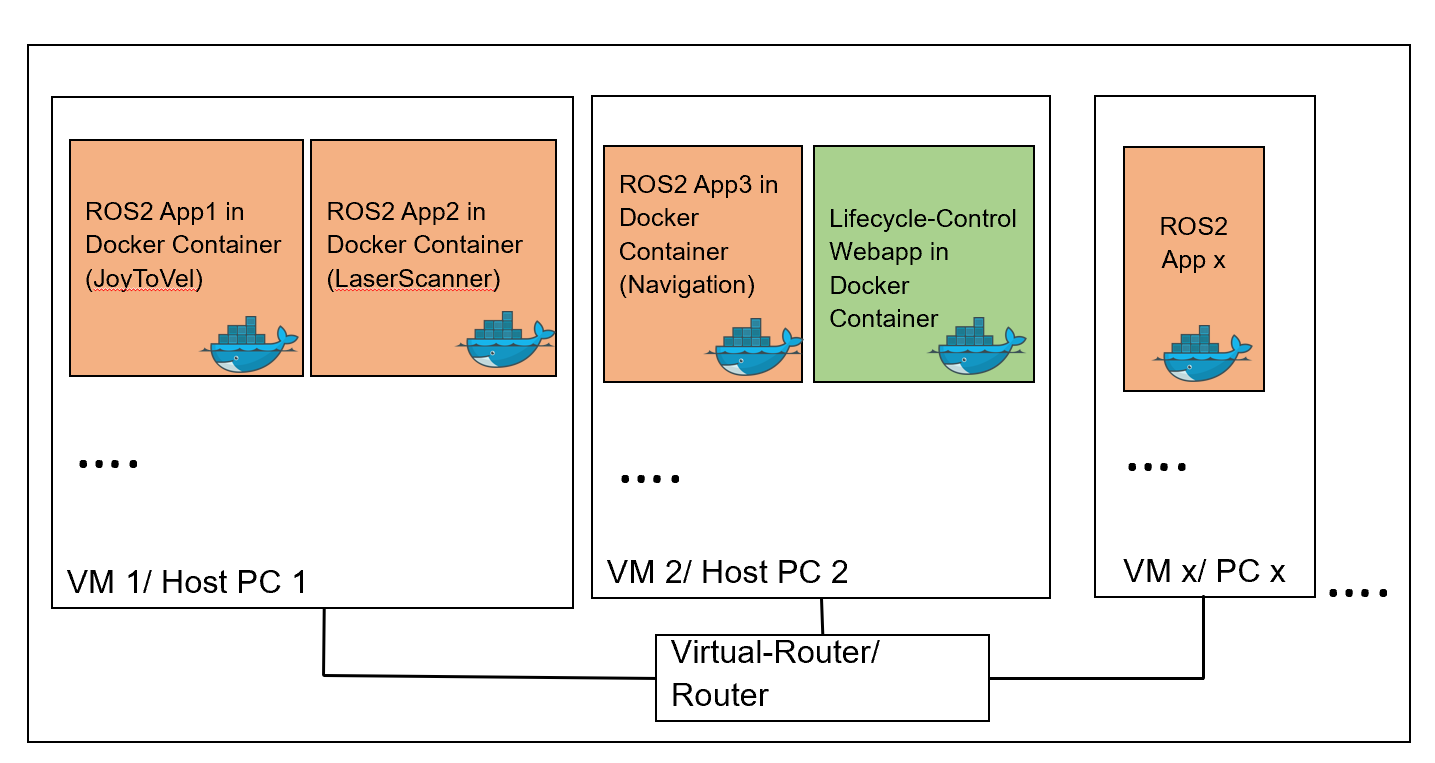
\includegraphics[width=0.95\textwidth]{"Bilder/Application-Structure.png"}
	\caption{Structure of Lifecycle Management Application}
	\label{fig:Background:LifecycleManagement}					
\end{figure}
The application consists of following major parts:

\begin{itemize}
	\item The Docker environment
	\item ROS2 Lifecycle Application
	\item Vue based Webinterface
	\item Integration
\end{itemize}

They will be explained in detail in the following section.

\section{The Docker environment}
\label{Implementierung:DockerEnvironment}
In order to develop an Industrial Edge Application, its necessary to pack an application into a Docker Image. Then it can be converted to an IE App using the Industrial Edge App Publisher.

This section describes the Docker image developed for the purposes of this thesis. A Dockerfile is used to define a Docker image. It consists of all the necessary software libraries and third party applications and precise order in which they have to installed. The following section will describe the details of the Dockerfile(structre of the Docker image) step by step.

\paragraph{Settng up the Base-Image} This is the first line in any Dockerfile. In this line the Ubuntu Ros Image to use is specified.
\begin{lstlisting}[language=docker,
	% caption={Dockerfile}, 
	label={code:DockerTestumgebung}]
	FROM ros:foxy-ros-core-focal
\end{lstlisting}


\paragraph{Installing Bootstrap Tools} This step installs the Bootstrap Tools(apt-utils, build-essentials, nano, git, curl, tmux) and necessary python3 extensions (python3-colcon-common-extensions, python3-colcon-mixin, python3-rosdep, python3-vcstool)

\begin{lstlisting}[language=docker,
	% caption={Dockerfile}, 
	label={code:DockerTestumgebung}]
	# install bootstrap tools
	RUN apt-get update && apt-get install -y --no-install-recommends \
		apt-utils \
		build-essential \
		nano \
		git \
		curl \
		tmux \
		inetutils-ping \
		python3-colcon-common-extensions \
		python3-colcon-mixin \
		python3-rosdep \
		python3-vcstool \
		&& rm -rf /var/lib/apt/lists/*

\end{lstlisting}

\paragraph{Setting up Ros Build environment} The rosdep is initialized and updated before installing any ROS2 Package. Then colcon mixin and metadata are setup and any relataed libraries are updated. Colcon is the default and recommended build system for ROS2. Now ROS2 applications can be built using colcon in the next step.
\begin{lstlisting}[language=docker,
	% caption={Dockerfile}, 
	label={code:DockerTestumgebung}]
	# bootstrap rosdep
	RUN rosdep init && \
	rosdep update --rosdistro $ROS_DISTRO
	# setup colcon mixin and metadata
	RUN colcon mixin add default \
		https://raw.githubusercontent.com/colcon/
		colcon-mixin-repository/master/index.yaml && \
		colcon mixin update && \
		colcon metadata add default \
		https://raw.githubusercontent.com/colcon/
		colcon-metadata-repository/master/index.yaml && \
		colcon metadata update
\end{lstlisting}

\paragraph*{Installimg necessary Ros packages} Following ROS2 Packages are instllen in this step: ros-foxy-ros-base=0.9.2-1*, ros-foxy-joy, ros-foxy-diagnostic-updater,ros-foxy-lifecycle. Depending on the type of ROS2 Appliation it might be necessary to install further Packages, which should be done in this to avoid furthr complications. Finally the system is updated to fix any broken installs and install any mising libraries.
\begin{lstlisting}[language=docker,
	% caption={Dockerfile}, 
	label={code:DockerTestumgebung}]
	# install ros2 packages
	RUN apt-get update && apt-get install -y --no-install-recommends \
		ros-foxy-ros-base=0.9.2-1* \
		ros-foxy-joy \
		ros-foxy-diagnostic-updater \
		# install for lifecycle 
		ros-foxy-lifecycle \
		nginx \
		python \
	# update system
		&& apt-get upgrade -y \
		&& rm -rf /var/lib/apt/lists/* 
\end{lstlisting}


\paragraph*{Sourcing Ros2} Sourcing is a common term among UNIX users. In order to make the desired changes applicable to the current shell , it is necessary to "source" the file. Furthermore adding sources to .bashrc files preconfigures any new shell opened. In this step ROS2 setup files are sourced so that other ROS2 commands can be run from the command line. 
\begin{lstlisting}[language=docker,
	% caption={Dockerfile}, 
	label={code:DockerTestumgebung}]
	#add sources to bashrc
	RUN echo "source /opt/ros/foxy/setup.bash" >> ~/.bashrc \
		&& echo "source /root/colcon_ws/install/setup.bash" >> ~/.bashrc
\end{lstlisting}

\paragraph*{Create and build Ros Workspace} In this step first of all the build workspaceis setup, then the necessary source files are copied from external working directory to the Docker internal workspace and finally built using colcon.
\begin{lstlisting}[language=docker,
	% caption={Dockerfile}, 
	label={code:DockerTestumgebung}]
	# create and build workspace
	ENV ROS2_WS /root/colcon_ws
		
	COPY ./evo_siemensrob_ctrl ${ROS2_WS}/src/evo_siemensrob_ctrl/.
	COPY ./joy_converter ${ROS2_WS}/src/joy_converter/.
	COPY ./joytovel ${ROS2_WS}/src/joytovel/.
	COPY ./twist_mux ${ROS2_WS}/src/twist_mux/.

	RUN cd ${ROS2_WS} \
		&& . /opt/ros/foxy/setup.sh \
		&& colcon build
		
	# install RIB support
	COPY ./RIBInstall .

	RUN ./RIBInstall \
		&& rm -rf RIBInstall
\end{lstlisting}

\paragraph{Setup Node enviroment for Vue} This step installs a version of NodeJS in this Docker environment. NodeJS will be necessary to build the Vue-application and run ros2-web-bridge in forthcoming steps. 
\begin{lstlisting}[language=docker,
	% caption={Dockerfile}, 
	label={code:DockerTestumgebung}]
	# For Lifecycle-Dashboard Vue App
	ENV NODE_VERSION=12.6.0
	# Already installed RUN apt install -y curl
	RUN curl -o- https://raw.githubusercontent.com/
	creationix/nvm/v0.34.0/install.sh | bash
	ENV NVM_DIR=/root/.nvm
	RUN . "$NVM_DIR/nvm.sh" && nvm install ${NODE_VERSION}
	RUN . "$NVM_DIR/nvm.sh" && nvm use v${NODE_VERSION}
	RUN . "$NVM_DIR/nvm.sh" && nvm alias default v${NODE_VERSION}
	ENV PATH="/root/.nvm/versions/node/v${NODE_VERSION}/bin/
	:${PATH}"
	RUN node --version
	RUN npm --version
\end{lstlisting}



\paragraph{Copy package.json files to install Node Project dependencies} A package.json file is a standard package specification file for NodeJS applications. It contains all the necessary configurations and list of packages to successfully build a NodeJS aplication. In this step 
a working directory for the Vue Application is created, the the package.json is copied to the Docker internal workdirectory and finally the project depencencies are downloaded and installed.
\begin{lstlisting}[language=docker,
	% caption={Dockerfile}, 
	label={code:DockerTestumgebung}]
	# build stage
	WORKDIR /app
	COPY ./lifecycle-dashboard/package*.json ./
	RUN npm install
\end{lstlisting}

\paragraph*{Build the web app for production} The project source files for the "Lifecycle management application" are copied from external workspace to the Docker workdirectory and built for production.
\begin{lstlisting}[language=docker,
	% caption={Dockerfile}, 
	label={code:DockerTestumgebung}]
	# build stage
	COPY ./lifecycle-dashboard/ .
	RUN npm run build
\end{lstlisting}

\paragraph{Setting up a Nginx web server} In this step the nginx configuration file is copied from external workspace to the docker enviroment. THe built application consisting of only .html, .css and .js files are copid to a location where nginx can easily find them and use them to start the web-application. Furthermore PORT 80 is exposed and the web-application can thus be accessed on locahost:8080 within the same network where this Docker container is running.
\begin{lstlisting}[language=docker,
	% caption={Dockerfile}, 
	label={code:DockerTestumgebung}]
	# For nginx
	COPY ./nginx.conf /etc/nginx/nginx.conf
	RUN cp -a /app/dist/. /var/www/html
	EXPOSE 80
\end{lstlisting}

\paragraph*{Installing ros2-web-bridge} In this step ros2-web-bridge is installed and other services that need to launch at startup are setup. The web-server(nginx) is setup to start at launch.
\begin{lstlisting}[language=docker,
	% caption={Dockerfile}, 
	label={code:DockerTestumgebung}]
	
	# install ros2-web-bridge

	# set workdirectory as /root
	WORKDIR /root

	#for automatic launch when container gets started 
	COPY ./dockerfile_startup.sh dockerfile_startup.sh
	RUN ["chmod", "+x", "./dockerfile_startup.sh"]
	CMD ./dockerfile_startup.sh	
\end{lstlisting}

\paragraph{Starting Ros Application} This step launches the installed ROS2-Application using its launchfile.
\begin{lstlisting}[language=bash,
	% caption={dockerfile_startup}, 
	label={code:DockerTestumgebung}]
	#!/bin/bash

	nginx
	. /opt/ros/foxy/setup.sh
	. /root/colcon_ws/install/setup.sh
	npm install ros2-web-bridge
	node node_modules/ros2-web-bridge/bin/rosbridge.js &
	ros2 launch evo_siemensrob_ctrl agv_control_launch.py 
\end{lstlisting}

\paragraph{Startup and Build scripts} Hh

% \begin{lstlisting}[language=html,
% 	caption={build_lifecycle.sh}, 
% 	label={code:DockerTestumgebung}]
% 	#!/bin/bash
% 	docker build . -t ubuntu_foxy:manual_control_rti
% 	docker run -it --privileged --network host --group-add dialout --ipc="host" --name agv_control_joy_rti ubuntu_foxy:manual_control_rti
% \end{lstlisting}

\begin{lstlisting}[language=html,
	% caption={run_lifecycle.sh}, 
	label={code:DockerTestumgebung}]
	#!/bin/bash
	docker start agv_control_joy_rti

	docker exec -it agv_control_joy_rti bash 
\end{lstlisting}

\section{ROS2 Lifecycle Application}
\label{Implementierung:ROS2LifecycleApplication} This section describes the details of an example ROS2-Application with managed states and steps necessary to convert a normal ROS2-node into a managed lifecycle node.     

\subsection{Conversion of a node into a Lifecycle Node}

\section{Vue based Webinterface}
\label{Implementierung:VueBasedWebinterface}
The developed web interface is supposed to be a web version of the lifecycle management CLI. 


% usage: ros2 lifecycle get [-h] [--spin-time SPIN_TIME] [--no-daemon][--include-hidden-nodes]                 [node_name]

% usage: ros2 lifecycle set [-h] [--spin-time SPIN_TIME] [--no-daemon]
%                           [--include-hidden-nodes]
%                           node_name transition

% Trigger lifecycle state transition

% positional arguments:
%   node_name             Name of the ROS node
%   transition            The lifecycle transition


%   usage: ros2 lifecycle list [-h] [--spin-time SPIN_TIME] [--no-daemon]
%   [--include-hidden-nodes] [-a]
%   node_name

% Output a list of available transitions

% positional arguments:
% node_name             Name of the ROS node

% ros2 lifecycle nodes [-h] [--spin-time SPIN_TIME] [--no-daemon] [-a]
%                             [-c]

% Output a list of nodes with lifecycle


% # Default values for transitions as described in:
% # http://design.ros2.org/articles/node_lifecycle.html

% # Reserved [0-9], publicly available transitions.
% # When a node is in one of these primary states, these transitions can be
% # invoked.

% # This transition will instantiate the node, but will not run any code beyond
% # the constructor.
% uint8 TRANSITION_CREATE = 0

% # The node’s onConfigure callback will be called to allow the node to load its
% # configuration and conduct any required setup.
% uint8 TRANSITION_CONFIGURE = 1

% # The node’s callback onCleanup will be called in this transition to allow the
% # node to load its configuration and conduct any required setup.
% uint8 TRANSITION_CLEANUP = 2

% # The node's callback onActivate will be executed to do any final preparations
% # to start executing.
% uint8 TRANSITION_ACTIVATE = 3

% # The node's callback onDeactivate will be executed to do any cleanup to start
% # executing, and reverse the onActivate changes.
% uint8 TRANSITION_DEACTIVATE = 4

% # This signals shutdown during an unconfigured state, the node's callback
% # onShutdown will be executed to do any cleanup necessary before destruction.
% uint8 TRANSITION_UNCONFIGURED_SHUTDOWN  = 5

% # This signals shutdown during an inactive state, the node's callback onShutdown
% # will be executed to do any cleanup necessary before destruction.
% uint8 TRANSITION_INACTIVE_SHUTDOWN = 6

% # This signals shutdown during an active state, the node's callback onShutdown
% # will be executed to do any cleanup necessary before destruction.
% uint8 TRANSITION_ACTIVE_SHUTDOWN = 7

% # This transition will simply cause the deallocation of the node.
% uint8 TRANSITION_DESTROY = 8

% # Reserved [10-69], private transitions
% # These transitions are not publicly available and cannot be invoked by a user.
% # The following transitions are implicitly invoked based on the callback
% # feedback of the intermediate transition states.
% uint8 TRANSITION_ON_CONFIGURE_SUCCESS = 10
% uint8 TRANSITION_ON_CONFIGURE_FAILURE = 11
% uint8 TRANSITION_ON_CONFIGURE_ERROR = 12

% uint8 TRANSITION_ON_CLEANUP_SUCCESS = 20
% uint8 TRANSITION_ON_CLEANUP_FAILURE = 21
% uint8 TRANSITION_ON_CLEANUP_ERROR = 22

% uint8 TRANSITION_ON_ACTIVATE_SUCCESS = 30
% uint8 TRANSITION_ON_ACTIVATE_FAILURE = 31
% uint8 TRANSITION_ON_ACTIVATE_ERROR = 32

% uint8 TRANSITION_ON_DEACTIVATE_SUCCESS = 40
% uint8 TRANSITION_ON_DEACTIVATE_FAILURE = 41
% uint8 TRANSITION_ON_DEACTIVATE_ERROR = 42

% uint8 TRANSITION_ON_SHUTDOWN_SUCCESS = 50
% uint8 TRANSITION_ON_SHUTDOWN_FAILURE = 51
% uint8 TRANSITION_ON_SHUTDOWN_ERROR = 52

% uint8 TRANSITION_ON_ERROR_SUCCESS = 60
% uint8 TRANSITION_ON_ERROR_FAILURE = 61
% uint8 TRANSITION_ON_ERROR_ERROR = 62

% # Reserved [90-99]. Transition callback success values.
% # These return values ought to be set as a return value for each callback.
% # Depending on which return value, the transition will be executed correctly or
% # fallback/error callbacks will be triggered.

% # The transition callback successfully performed its required functionality.
% uint8 TRANSITION_CALLBACK_SUCCESS = 97

% # The transition callback failed to perform its required functionality.
% uint8 TRANSITION_CALLBACK_FAILURE = 98

% # The transition callback encountered an error that requires special cleanup, if
% # possible.
% uint8 TRANSITION_CALLBACK_ERROR = 99

% ##
% ## Fields
% ##

% # The transition id from above definitions.
% uint8 id

% # A text label of the transition.
% string label

\begin{figure}[H]
	\centering
	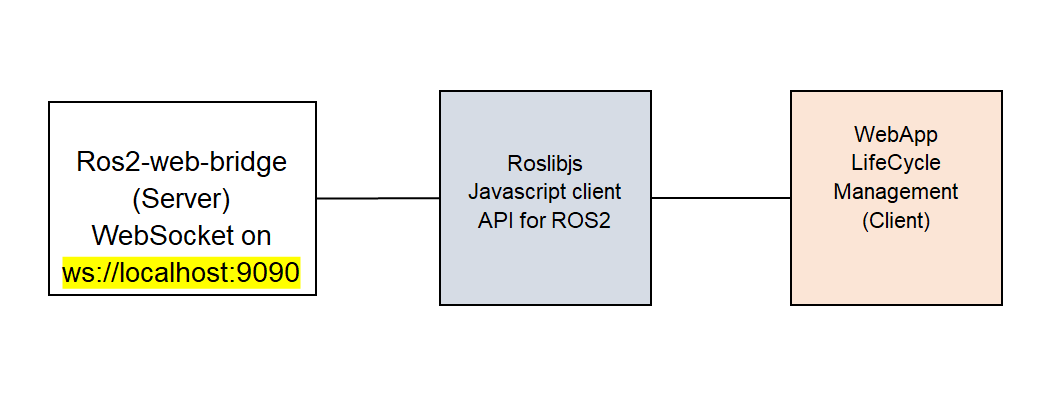
\includegraphics[width=0.95\textwidth]{"Bilder/webapp-design.png"}
	\caption{Overview of Lifecycle Management WebApp}
	\label{fig:Background:WebappDesign}					
\end{figure}


\subsection{ROS2 Message Types/ Javascript Objects}

\subsection{ROS2 Javascript Functions}

\begin{lstlisting}[language=JavaScript,
	% caption={dockerfile_startup}, 
	label={code:Vue}]
	
	import * as ROSLIB from 'roslib';
	import { MDBBtn, MDBBtnGroup, MDBInput, MDBContainer, MDBRow, MDBCol } from "mdb-vue-ui-kit";

	export default {
	
	name: 'LifecycleManagement',
	components: {
		MDBBtn, MDBBtnGroup, MDBInput, MDBContainer, MDBRow, MDBCol
	},
	props: {
		msg: String,
	},
	data: function () {
		return {
		unsub: false,
		console_out: [],
		selected_logger_level: 20,
		input_node_name:"",
		added_nodes:["lifecycle_joytovel"],
		active_node: "lifecycle_joytovel",
		selected_transition: {},
		available_states: [],
		available_transitions: [],
		current_state: {},
		ros: new ROSLIB.Ros({
			url : 'ws://localhost:9090'
		})
		}
	},
	
	mounted: function () {
		var ros = new ROSLIB.Ros({
			url : 'ws://localhost:9090'
		});

		ros.on('connection', function() {
			console.log('Connected to websocket server.');
		});

		ros.on('error', function(error) {
			console.log('Error connecting to websocket server: ', error);
		});

		ros.on('close', function() {
			console.log('Connection to websocket server closed.');
		});

		this.update();
	},

	methods: {

		// Available Services :
		// /lifecycle_joytovel/change_state
		// /lifecycle_joytovel/describe_parameters
		// /lifecycle_joytovel/get_available_states
		// /lifecycle_joytovel/get_available_transitions
		// /lifecycle_joytovel/get_parameter_types
		// /lifecycle_joytovel/get_parameters
		// /lifecycle_joytovel/get_state
		// /lifecycle_joytovel/get_transition_graph
		// /lifecycle_joytovel/list_parameters
		// /lifecycle_joytovel/set_parameters
		// /lifecycle_joytovel/set_parameters_atomically
		clear() {
			this.available_states = [];
			this.current_state = [];
			this.available_transitions = [];
		},
		update() {
			this.srvGetCurrentState()
			this.srvGetAvailableTransitions()
			this.srvGetAvailableStates()
		},

		dynobtn(par){
		console.log(par);
		},

		add_node(){
			if (this.input_node_name !== "") {
				this.added_nodes.push(this.input_node_name);
				console.log(this.added_nodes);
			} 
		},

		set_active_node(data){
			this.active_node = data;
			this.clear();
			this.update();
		},
		
		srvGetCurrentState() {
		var lifecycleClient = new ROSLIB.Service({
			ros : this.ros,
			// name : `/lifecycle_joytovel/get_state`,
			name : `/${this.active_node}/get_state`,
			serviceType : 'lifecycle_msgs/GetState'
		});

		console.log('Calling Service');
		var request = new ROSLIB.ServiceRequest({});
		console.log('Result for service call on '
			+ lifecycleClient.name
			+ ': ');
			lifecycleClient.callService(request, (result) => {
				console.log(result);
				this.current_state = result.current_state;
			})
		
		},

		
		srvGetAvailableStates() {
		var lifecycleClient = new ROSLIB.Service({
			ros : this.ros,
			name : `/${this.active_node}/get_available_states`,
			// name : '/lifecycle_joytovel/get_available_states', 
			serviceType : 'lifecycle_msgs/GetAvailableStates'
		});

		console.log('Calling Service srvGetAvailableStates');
		var request = new ROSLIB.ServiceRequest({});

		var tempArr = [];
		lifecycleClient.callService(request, (result) => {
			console.log(result);
			result.available_states.forEach(element => {
				console.log(element);
				tempArr.push(element);
			});
			this.available_states = tempArr;
		})

		console.log("this.available_states");
		},

	srvGetAvailableTransitions() {
		var lifecycleClient = new ROSLIB.Service({
			ros : this.ros,
			name : `/${this.active_node}/get_available_transitions`,
			// name : '/lifecycle_joytovel/get_available_transitions', 
			serviceType : 'lifecycle_msgs/GetAvailableTransitions'
		});

		console.log('Calling Service srvGetAvailableTransitions');
		var request = new ROSLIB.ServiceRequest({});

		var tempArr = [];
		
		lifecycleClient.callService(request, (result) => {
			console.log(result);
			result.available_transitions.forEach(element => {
				console.log(element);
				tempArr.push(element);
			});
			this.available_transitions = tempArr;
		})

		console.log(this.available_transitions);
		},

		srvChangeState() {
		var lifecycleClient = new ROSLIB.Service({
			ros : this.ros,
			name : `/${this.active_node}/change_state`,
			// name : '/lifecycle_joytovel/change_state', 
			serviceType : 'lifecycle_msgs/ChangeState'
		});

		console.log('Calling Service change_state');
	
		var r_id = parseInt(this.selected_transition);
		console.log(r_id );

		var request = new ROSLIB.ServiceRequest({
			transition: {id: r_id, label : ""}
		});

		lifecycleClient.callService(request, function(result) {
			console.log('Result for service call on '
			+ lifecycleClient.name);
			console.log(request);
			console.log(result);
		}, function(result) {
			console.log('Error');
			console.log(result);
		});
		this.update();
		},

		subscribeToRosOut(){
		var listener = new ROSLIB.Topic({
			ros : this.ros,
			name : '/rosout',
			messageType : 'rcl_interfaces/msg/Log'
			});
			var msg = [];
			listener.subscribe((msg)=> {
			this.console_out.push(msg);
			if (this.console_out.length > 10) {
				this.console_out.shift();
			}
			console.log(msg);
			if (this.unsub) {
				listener.unsubscribe();
			}
			}) 
			console.log(msg);
		},

		mapLogLevel(level){
		if (level === 30) {
			return "WARN"
		} else {
			return "INFO"
		}

		}
	},
\end{lstlisting}

\begin{figure}[H]
	\centering
	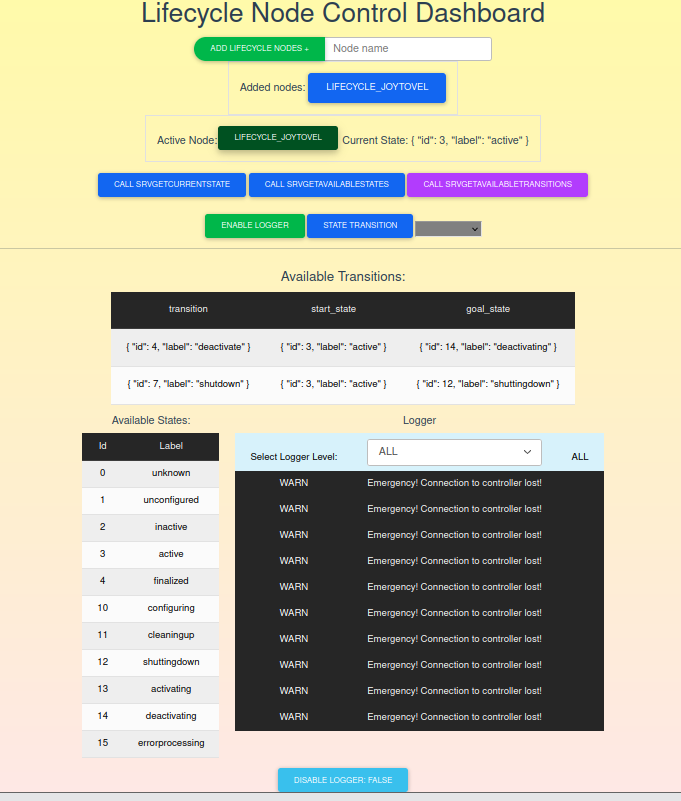
\includegraphics[width=0.95\textwidth]{"Bilder/lifecycle-dashboard.png"}
	\caption{Lifecycle Dashboard}
	\label{fig:Background:LifecycleDashboard}					
\end{figure}

\section{Integration}
\label{Implementierung:Integration}


	
		
		
	
	